\documentclass[12pt,a4paper]{article}
\usepackage[utf8]{inputenc}

\usepackage{mathtools}
\usepackage{amsmath}
\usepackage{amssymb}
\usepackage{amsthm}
\usepackage{amssymb}
\usepackage{mathdots}
\usepackage[pdftex]{graphicx}
\usepackage{fancyhdr}
\usepackage[margin=1in]{geometry}
\usepackage{multicol}
\usepackage{bm}
\usepackage{listings}
\usepackage{xcolor}
\usepackage{pdfpages}
\usepackage{algpseudocode}
\usepackage{tikz}
\usepackage{enumitem}
\usepackage[T1]{fontenc}
\usepackage{inconsolata}
\usepackage{framed}
\usepackage{wasysym}
\usepackage[thinlines]{easytable}
\usepackage{hyperref}
\usepackage{minted}
\usemintedstyle{perldoc}
\hypersetup{
    colorlinks=true,
    linkcolor=blue,
    filecolor=magenta,      
    urlcolor=blue,
}
\definecolor{codegreen}{rgb}{0,0.6,0}
\definecolor{codegray}{rgb}{0.5,0.5,0.5}
\definecolor{codepurple}{rgb}{0.58,0,0.82}
\definecolor{backcolour}{rgb}{0.95,0.95,0.92}
\lstdefinestyle{mystyle}{
    backgroundcolor=\color{backcolour},   
    commentstyle=\color{codegreen},
    keywordstyle=\color{magenta},
    numberstyle=\tiny\color{codegray},
    stringstyle=\color{codepurple},
    basicstyle=\ttfamily,
    breakatwhitespace=false,         
    breaklines=true,                 
    captionpos=b,                    
    keepspaces=true,                 
    numbers=left,                    
    numbersep=5pt,                  
    showspaces=false,                
    showstringspaces=false,
    showtabs=false,                  
    tabsize=4
}
\lstset{style=mystyle}
\newcommand\numberthis{\addtocounter{equation}{1}\tag{\theequation}}
\newcommand{\rightqed}{
\begin{flushright}
$\blacksquare$
\end{flushright}
}
\newcommand{\solution}{\noindent\textbf{Solution:}\\\indent}
\usepackage{graphics}
\usepackage{subfig}
\graphicspath{ {./images/} }

\title{6550 Artificial Intelligence Homework 2}
\author{Kushajveer Singh}
\date{}

\begin{document}
\maketitle

\subsection*{Problem 1}

\begin{figure}[H]
    \centering
    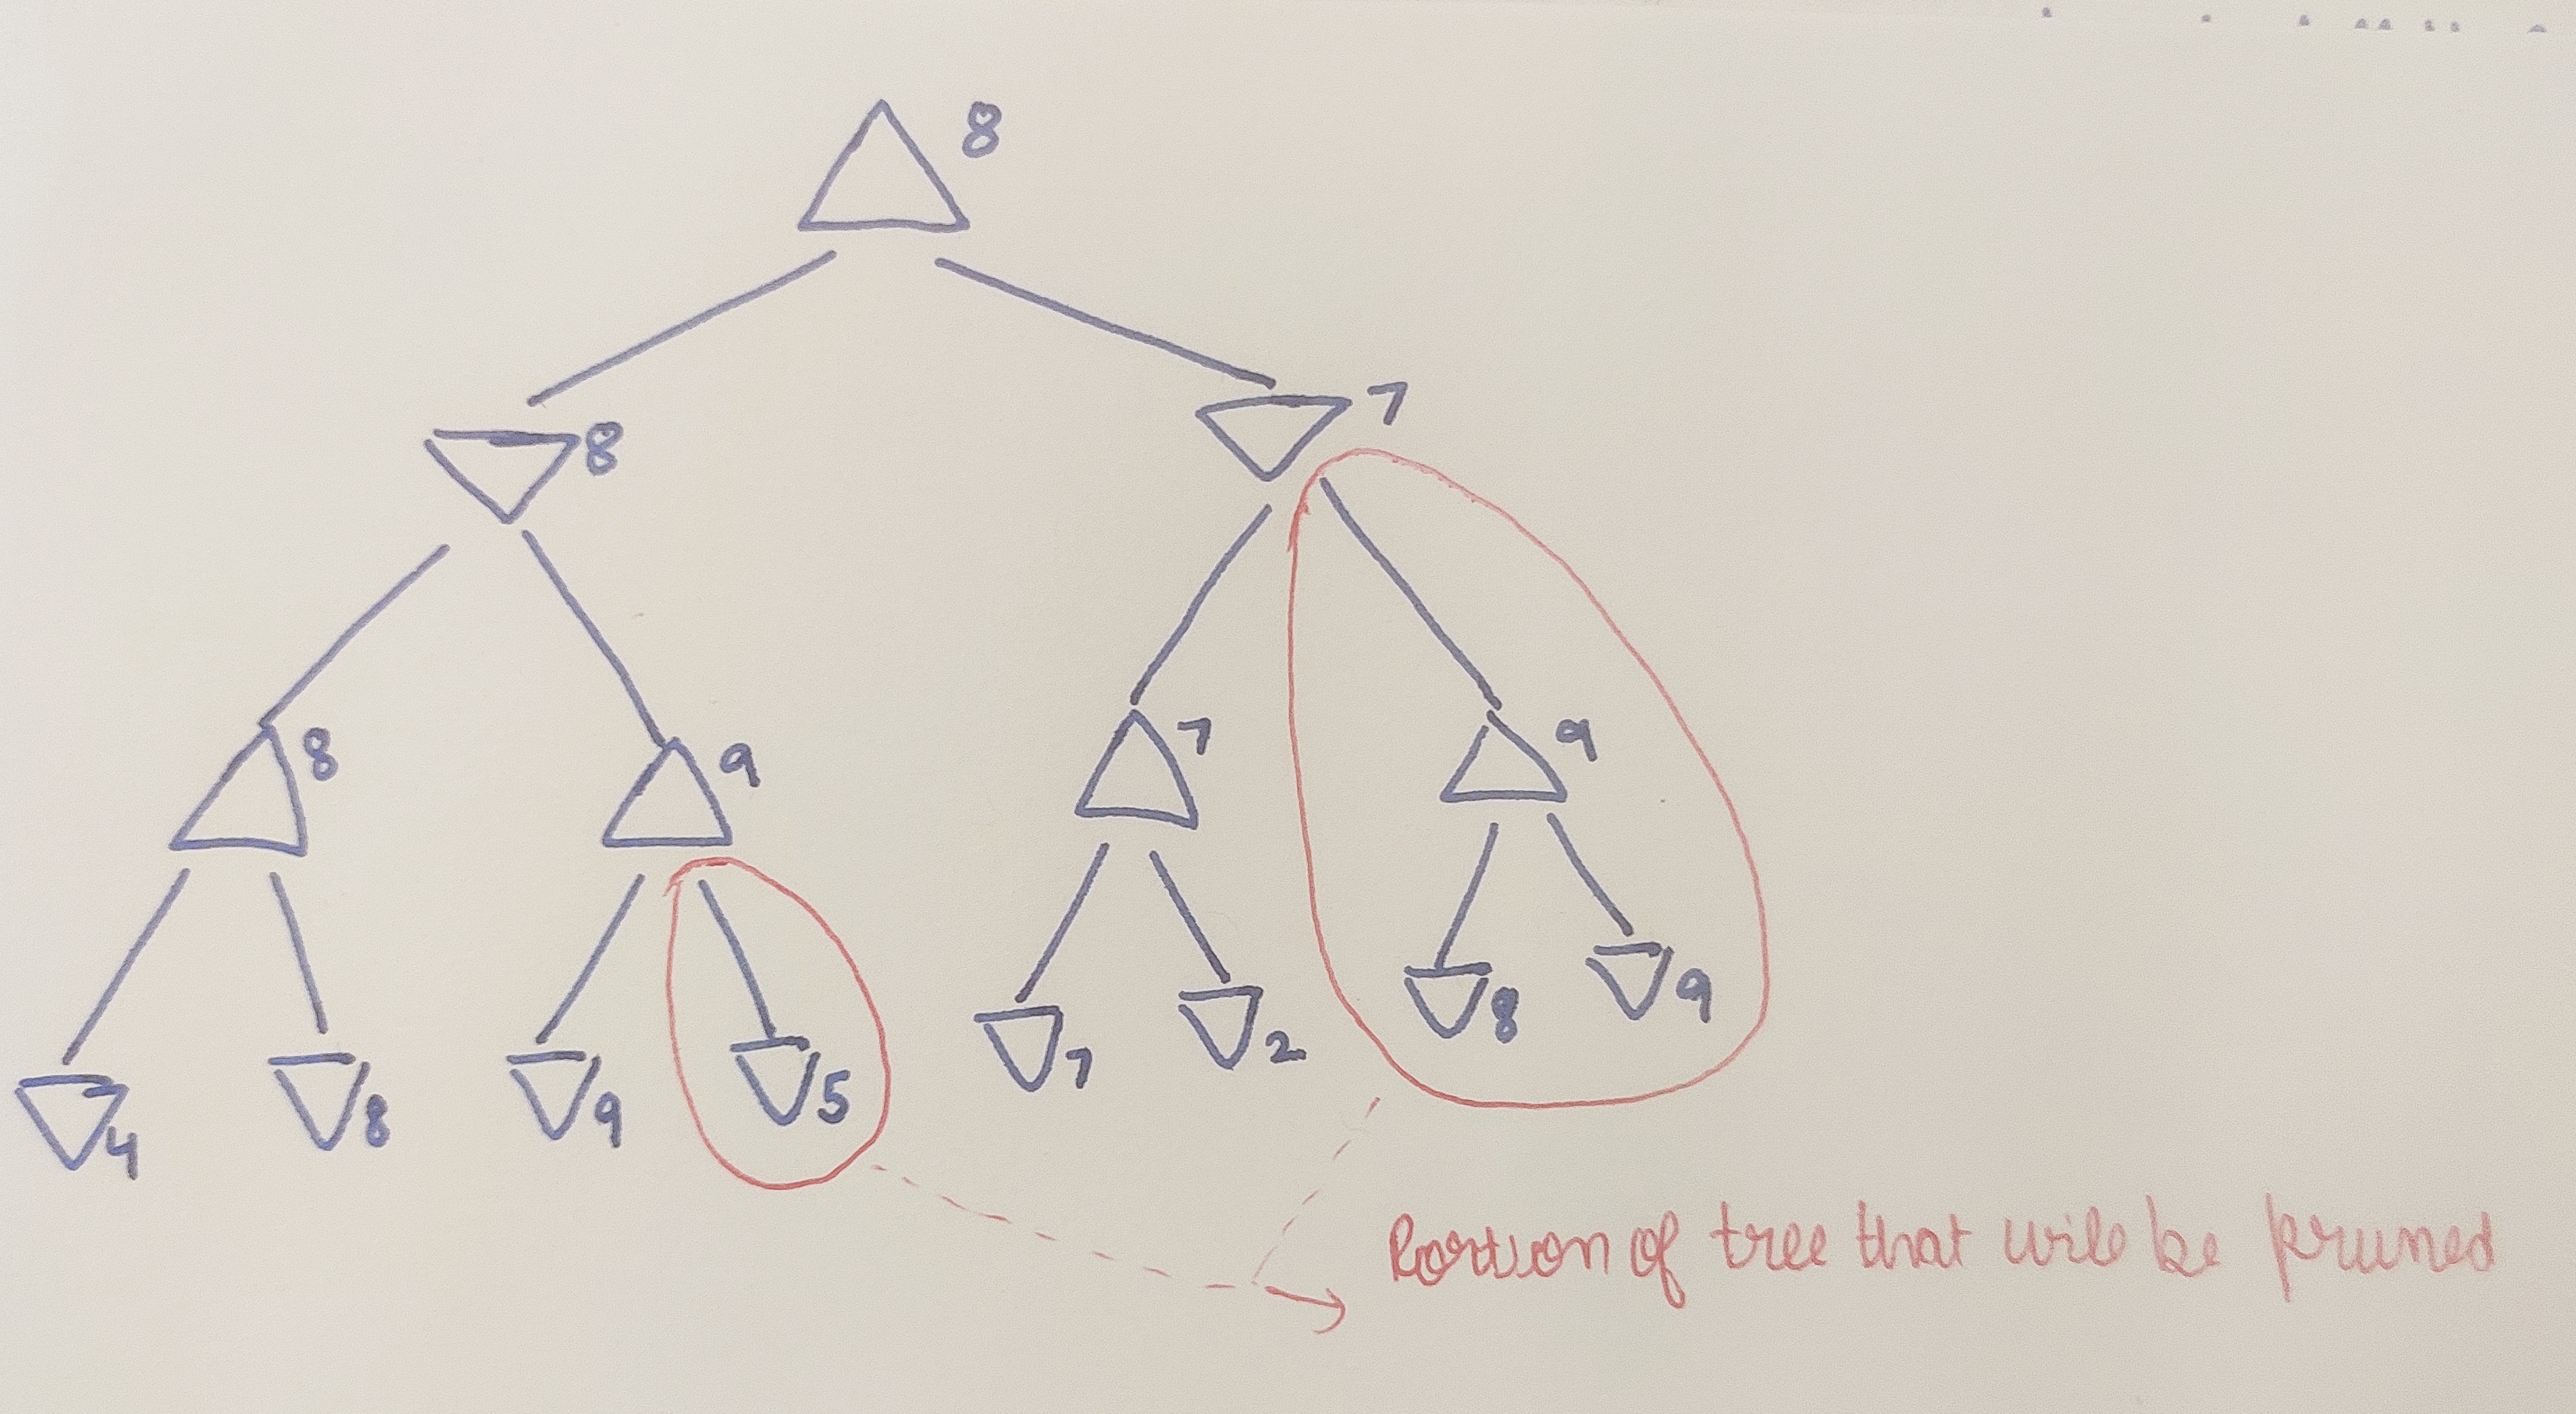
\includegraphics[width=13cm]{prob1.jpg}
    \caption{minimax tree (MAX goes first)}
\end{figure}

\subsection*{Problem 2}

\begin{figure}[H]
    \centering
    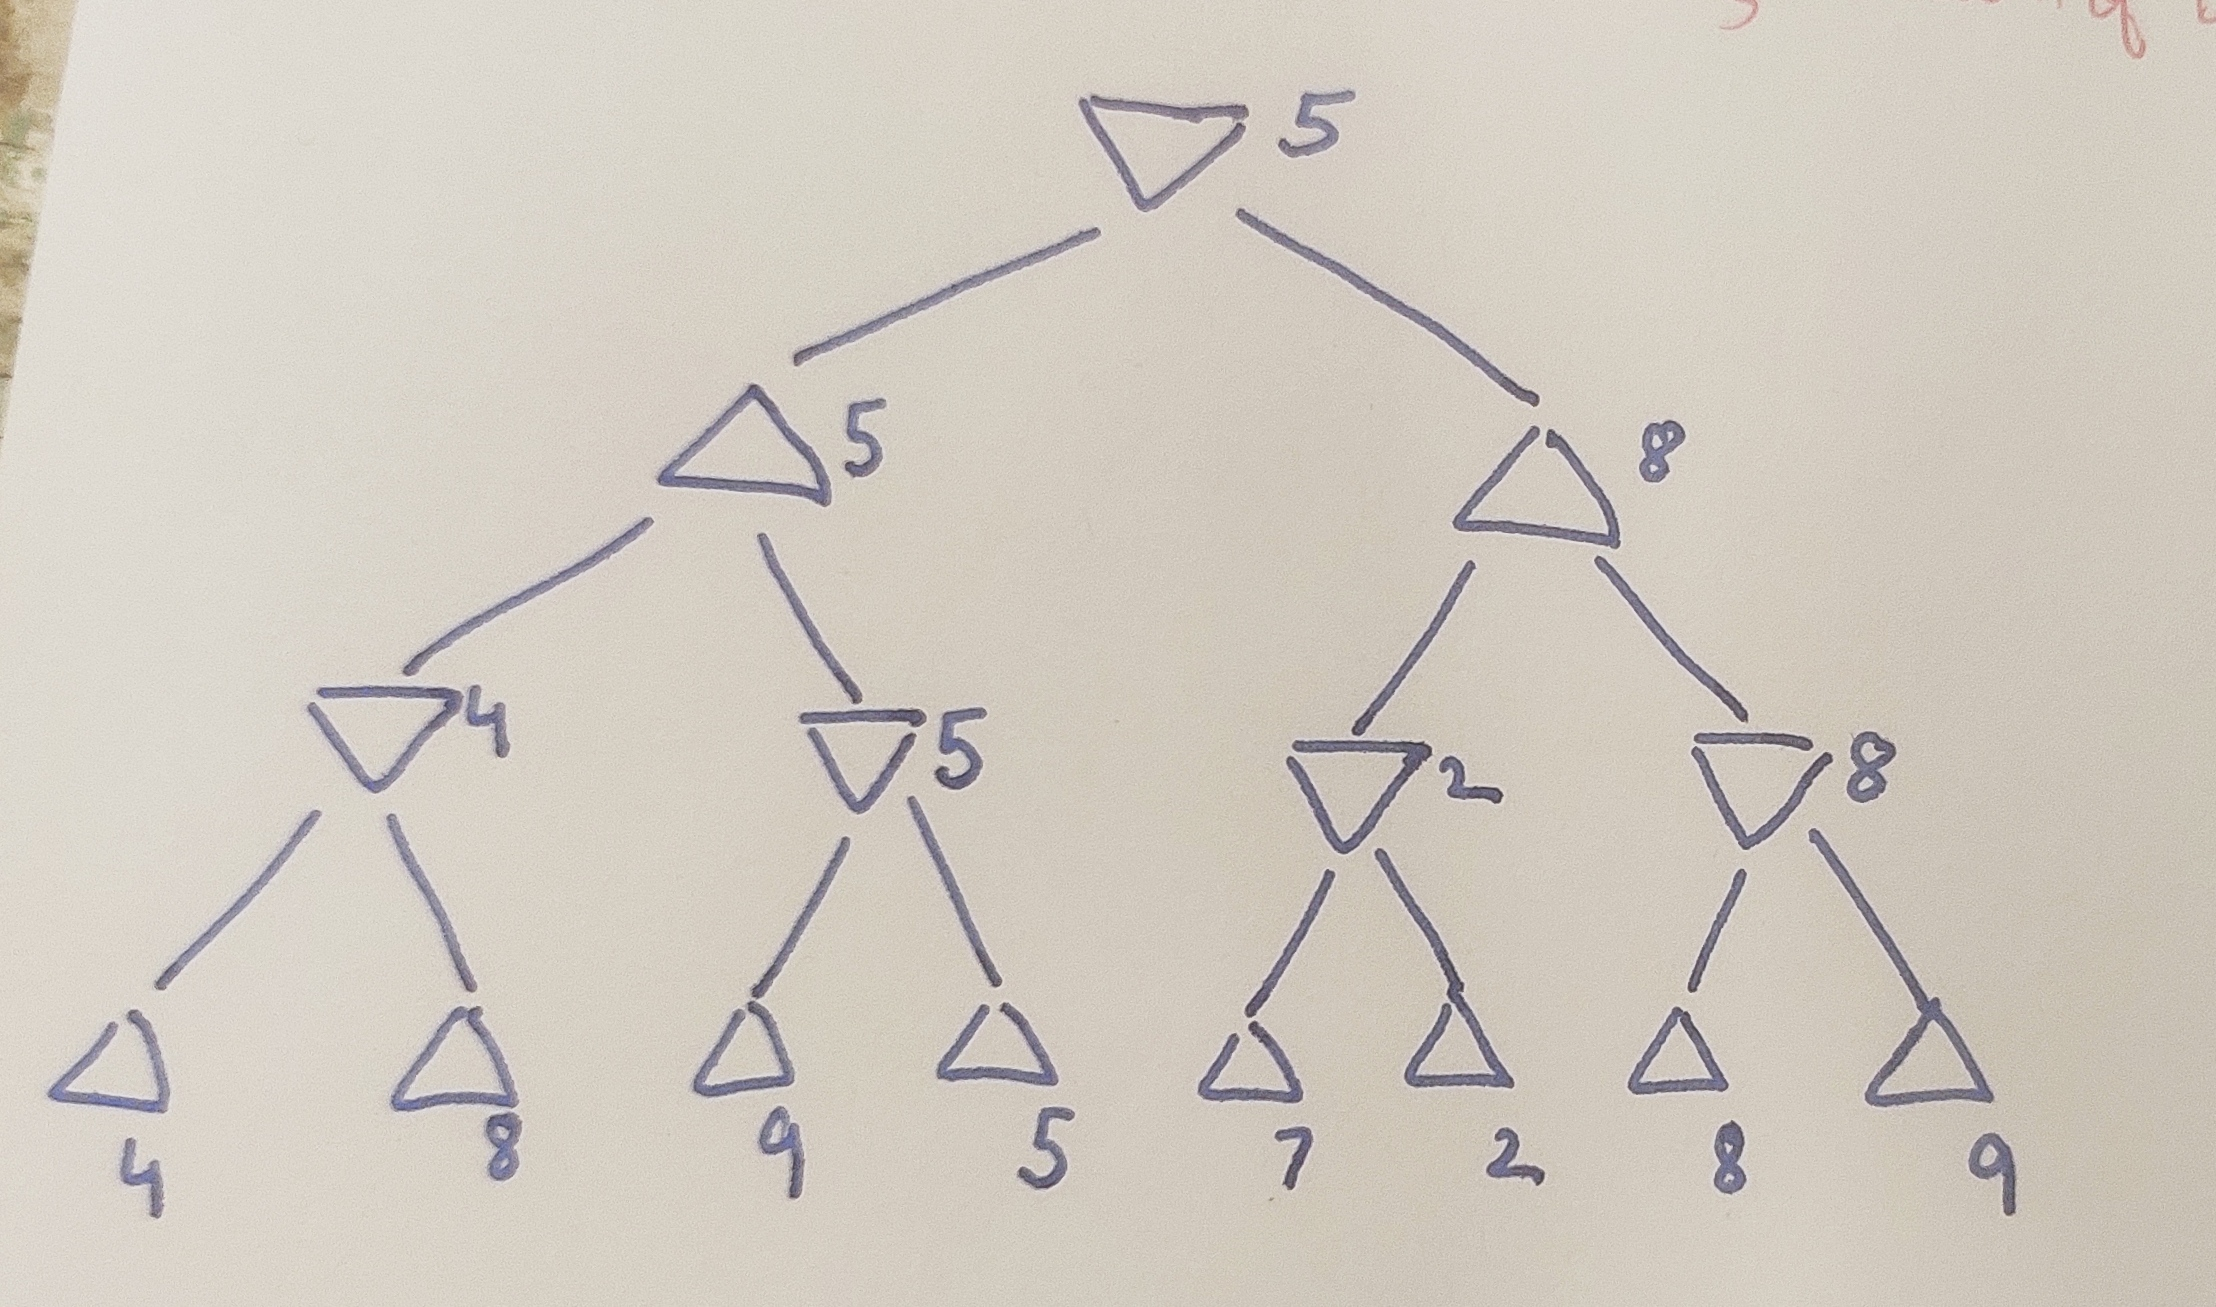
\includegraphics[width=14cm]{prob2.jpg}
    \caption{minimax tree (MIN goes first)}
\end{figure}

\subsection*{Problem 3}

\begin{figure}[H]
    \centering
    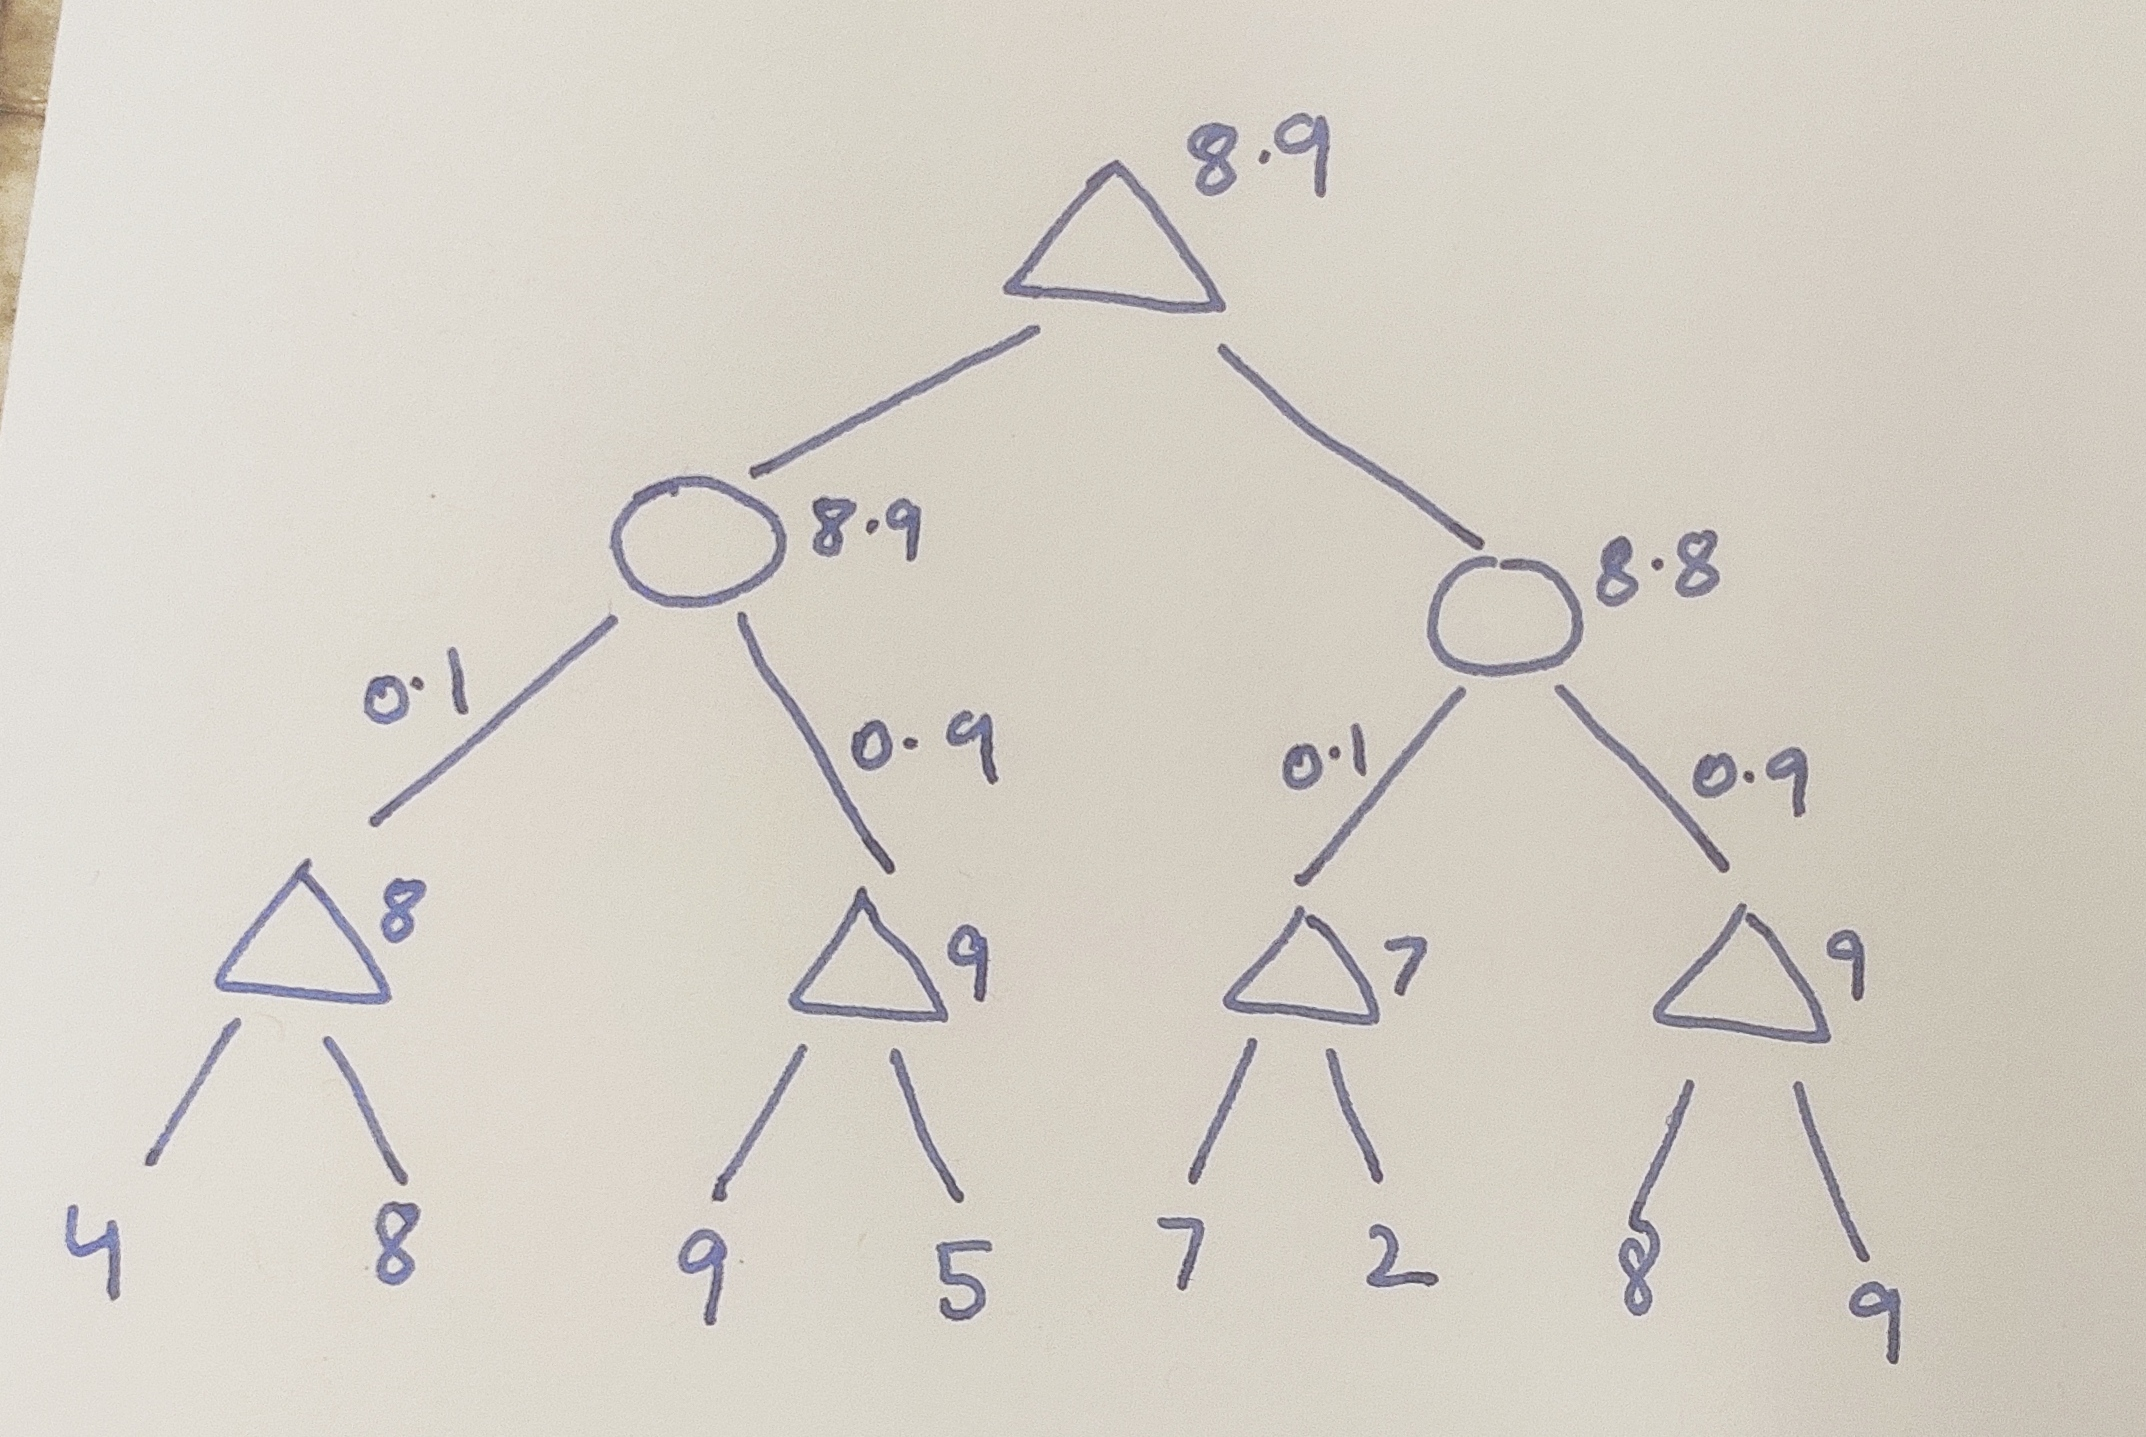
\includegraphics[width=13cm]{prob3.jpg}
    \caption{minimax tree (MIN plays randomly)}
\end{figure}

In this case, MAX cannot come up with an optimal solution (sequence of actions) to win the game because the other player may not play rationally (as the moves picked by the other player are random). Therefore, MAX has to come up with a strategy that is most likely to win the game and the strategy has to deal with the stochastic nature of other player.


\subsection*{Problem 4}

\begin{figure}[H]
    \centering
    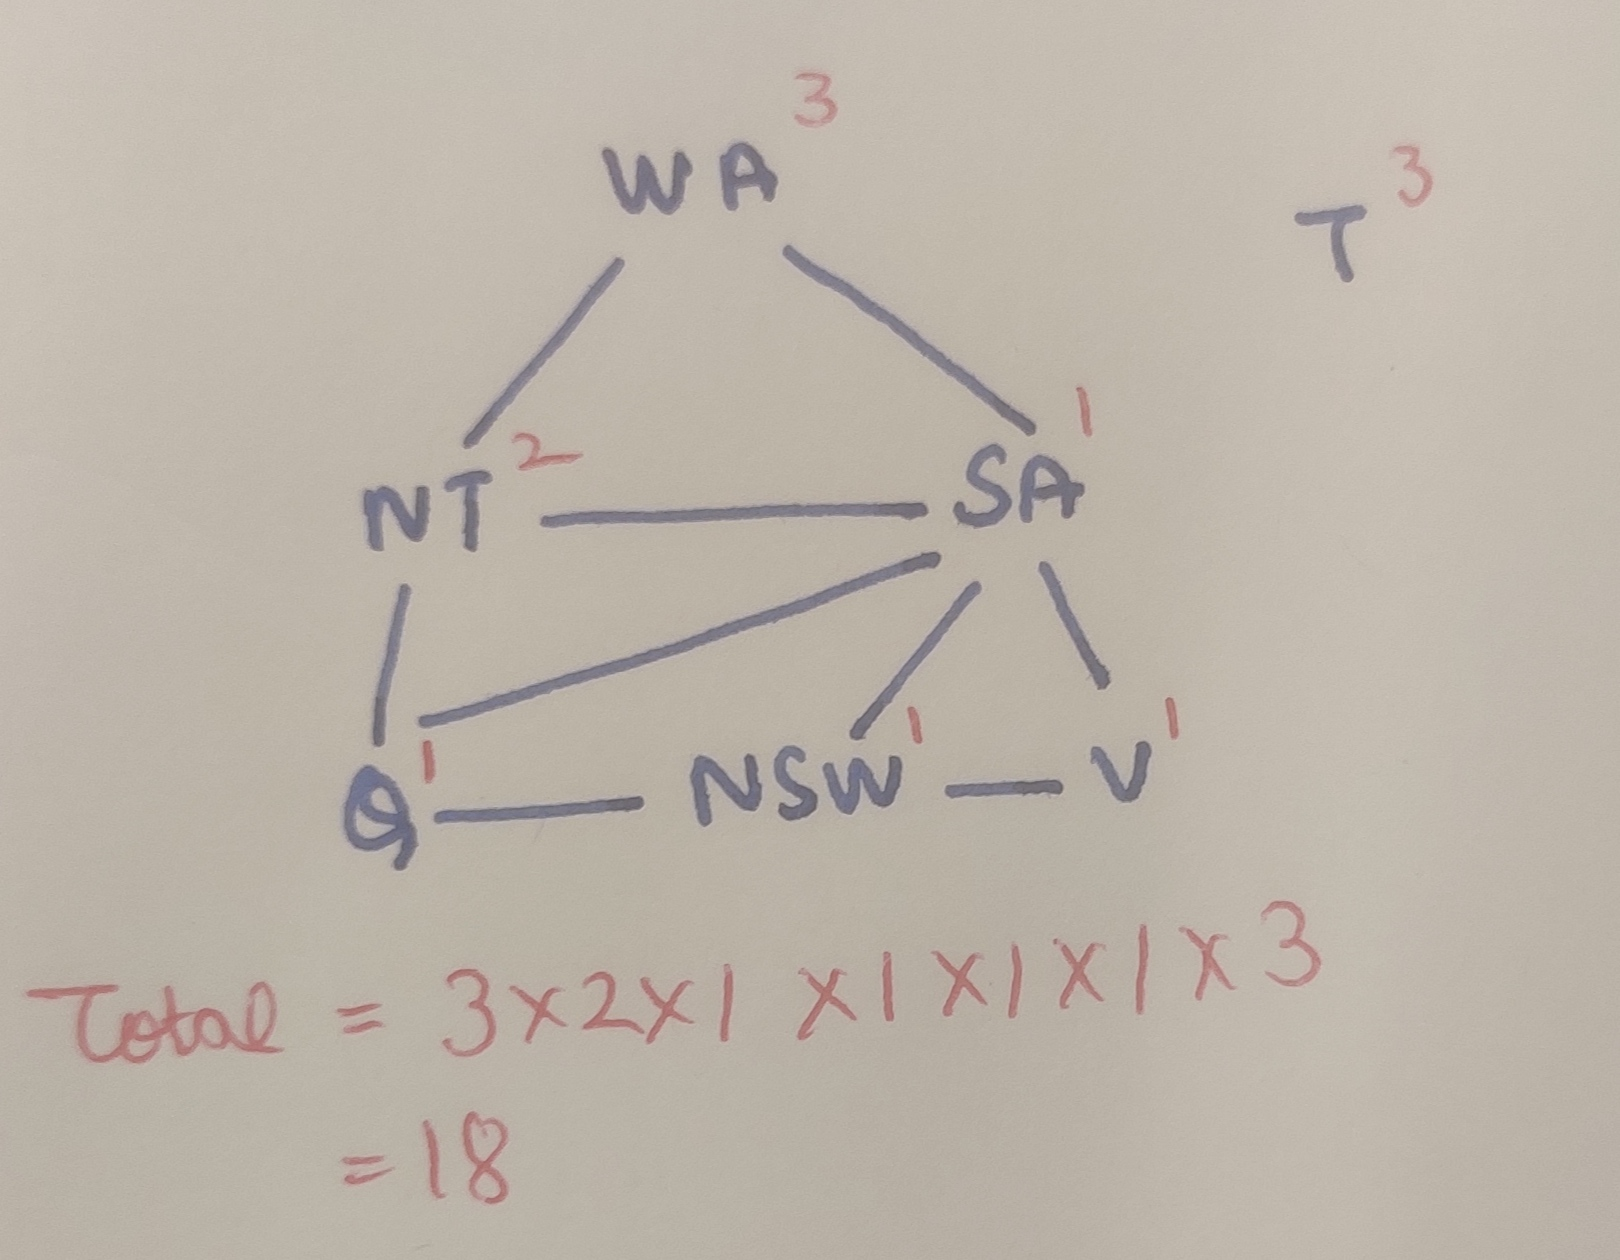
\includegraphics[width=10cm]{prob4_1.jpg}
    \caption{3-colors}
\end{figure}

In case of 3 colors, there are 18 different solutions for the map-coloring problem. If we pick WA as starting node. Then WA can be colored in 3 ways. Then NT can be colored in 2 ways and SA can be colored in 1 way (as NT and SA are connected). As NT and SA have different color, Q can be colored in only 1 way and then NSW and V follow the same reasoning.

\begin{figure}[H]
    \centering
    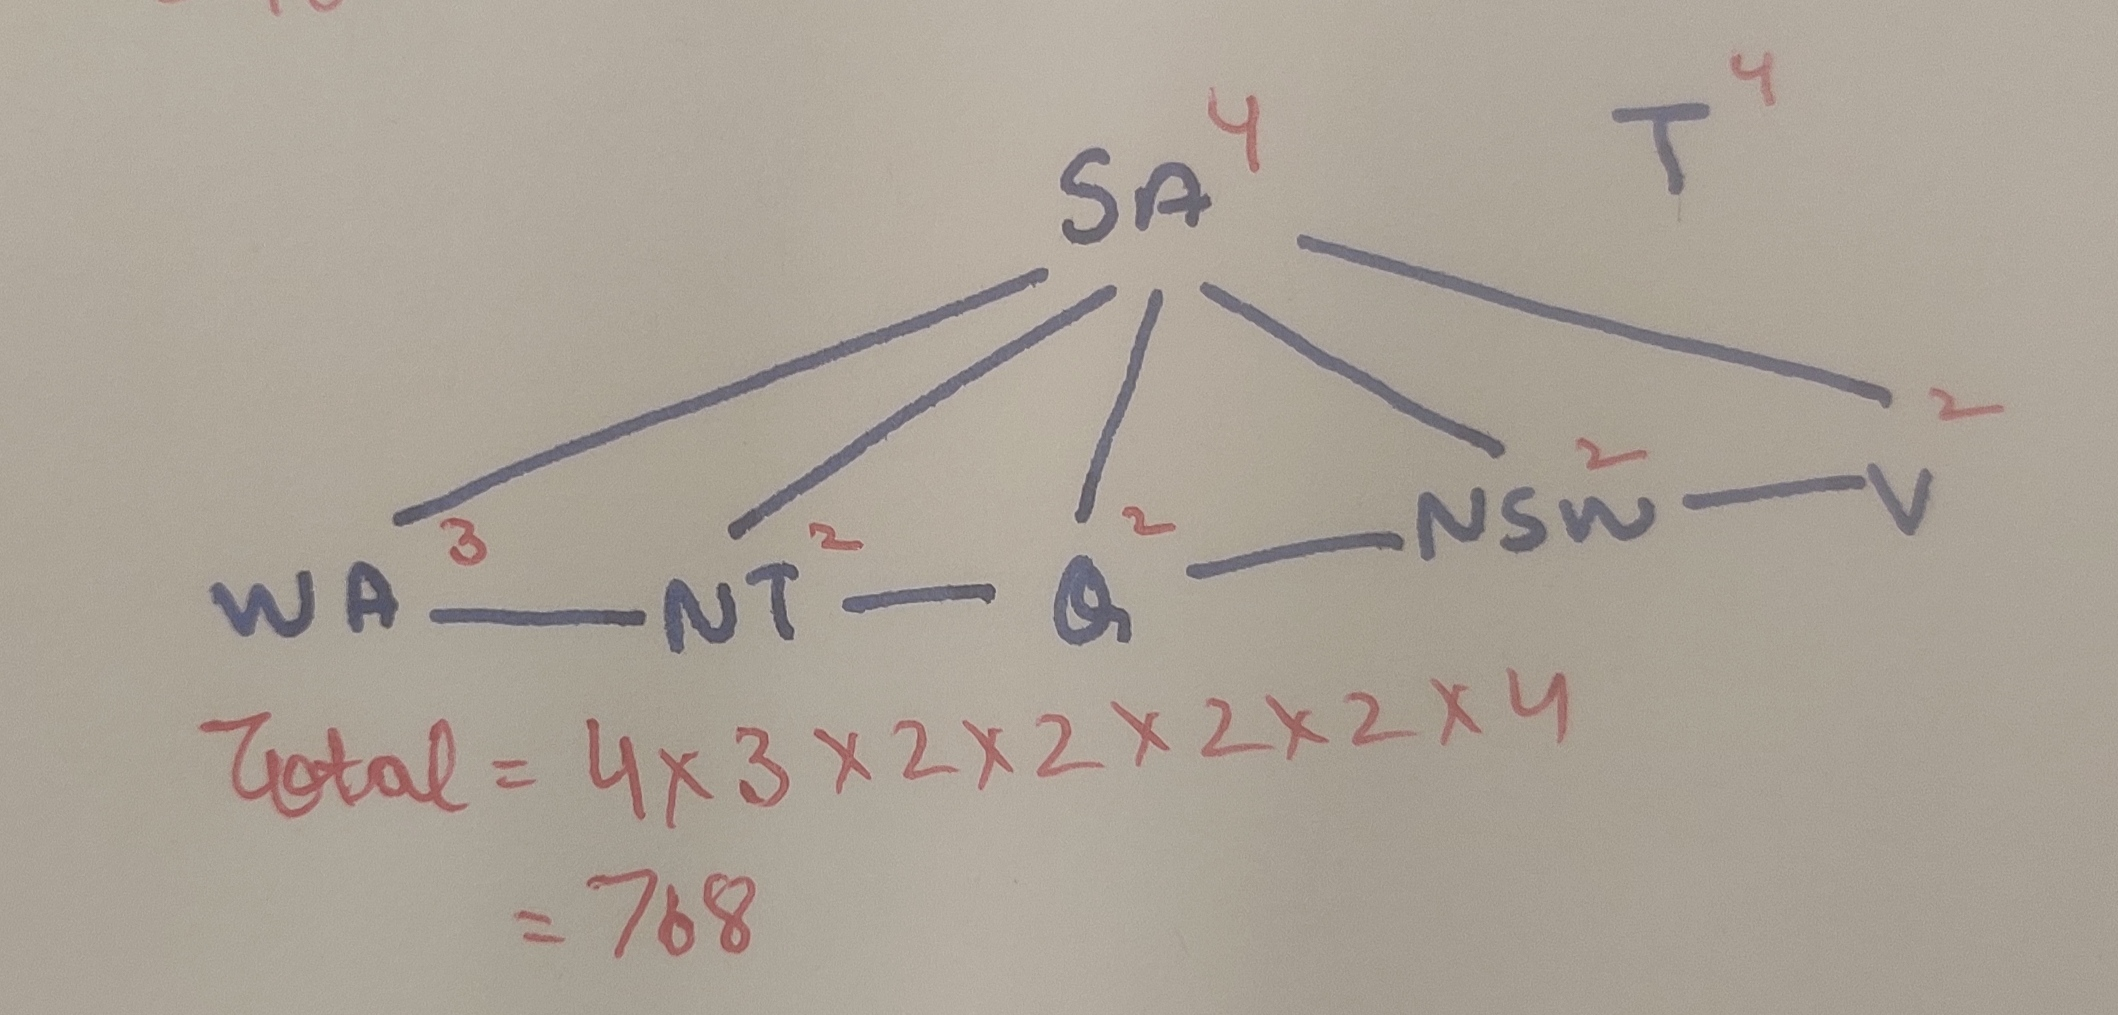
\includegraphics[width=10cm]{prob4_2.jpg}
    \caption{4-colors}
\end{figure}

In case of 4 colors, there are 768 different solutions for the map-coloring problem. Starting with SA, we can can color it in 4 ways. Then WA can be colored in 3 ways and NT in 2 ways (as WA and NT are connected). Now Q is connected to SA and NT, which means it can only take 2 colors. For NSW, it is connected to SA and Q which means it can take 2 colors and same for V.

In case of 2 colors, there are 0 solutions. If we assign the first color to SA and the second color to WA, then we do not have any color left to color NT as NT must have a different from SA and WA.

\subsection*{Problem 5}

Initial domain of all nodes before using AC-3 algorithm
\begin{itemize}
    \item WA = \{green\}
    \item V = \{red\}
    \item SA = \{red, green, blue\}
    \item NT = \{red, green, blue\}
    \item Q = \{red, green, blue\}
    \item NSW = \{red, green, blue\}
    \item T = \{red, green, blue\}
\end{itemize}

The agenda (queue) contains all the constraints in both directions i.e. both $WA \neq SA$ and $SA \neq WA$ will be in the agenda. Showing some of the constraints in the agenda

Agenda
\begin{itemize}
    \item $WA \neq SA$
    \item $SA \neq WA$
    \item $SA \neq V$
    \item $V \neq SA$
    \item $WA \neq NT$
    \item $NT \neq WA$
    \item ...
\end{itemize}

The AC-3 algorithm will operate as follows
\begin{itemize}
    \item Pop $WA \neq SA$ from agenda. Now every value in domain of WA = \{green\} can be satisfied by some value in domain of SA (e.g. SA = red). As there is no change in domain of WA we continue.
    \item Pop $SA \neq WA$ from the agenda. Now every value in domain of SA cannot be satisfied by some value in domain of SA (i.e. SA = green is not valid under the given constraint), so we remove green from the domain of SA. As domain of SA is changed we need to add all the constraints that have SA on the right (and that are not in the agenda). In our case, we only need to add $WA \neq SA$ to the agenda.
    \item Pop $SA \neq V$ from the agenda. We need to remove red from the domain of SA so as to satisfy the constraint, we need to add all the constraints with SA on the right to the agenda. In this, case all the constraints are already in the agenda so no need to add them again.
    \item continue till agenda is empty
\end{itemize}

The above steps show how the AC-3 algorithm can be used to detect the inconsistency of the partial assignment \{WA = green, V = red\}.

\subsection*{Problem 5}

Clustering Illusion is the intuition that random events such as coin flips should alternate between heads and tails more than they do. Random distributions seem to us to have too many clusters or streaks of consecutive outcomes of the same type, and so we have difficulty accepting their true origins.

Streak shooting can be attributed to people's tendency to be overly influenced by judgments of "representativeness" i.e. the reflexive tendency to assess the similarity of outcomes, instances, and categories on relatively salient and even superficial features, and then to use these assessments of similarity as a basis of judgment.

Judgment by Representativeness is the phenomenon by which people chronically misconstrue random events, and that there may be other cases in which truly random phenomenon are erroneously thought to be ordered and "real".

Streak shooting can be attributed to the overapplication of representativeness i.e. all else is not always equal. People forget that law of averages only comes into play after a large number of outcomes and it is this over-generalization that leads to people believeing in streak shooting.

\subsection*{Problem 6}

When out beliefs and expectations influence our behavior at the subconscious level, is termed as self-fulfilling prophecy. For instance, behaving in an unfriendly and defensive manner because you think someone is hostile will generally produce the very hostility that was originally feared.

Seemingly self-fulfilling prophesy  refer to the expectations that alter another person's world, or limit another's responses, in such a way that is difficult or impossible for the expectations to be disconfirmed. Thus the expectancy is confirmed, not by the target person actively conforming to some expectancy, but by the target person having little opportunity to disconfirm.

This is an example of a hidden data problem because a perceiver's expectation can cause him or her to behave in such a way that certain behaviors by the target person cannot be observed, making what is observed a biased and misleading indicator of what that person is like.

\end{document}